\chapter{Test Results}

THIS APPENDIX HAS REFERENCES TO THE TEST SECTION OF THE REPORT

AND ASSUMES THE READER HAS KNOWLEDGE OF THE RIG DESIGN

This appendix contains the different tests, that have been conducted on the \gls{nxt} motors.

\section{Positive Brake Test}
This test examines the time each motor takes to brake, after it has been instructed to move a full rotation of 360\degree\ in a clockwise direction. The result is given by the number degrees the motor has moved further than the instructed 360\degree . And will consider the consistency of each motor.

\subsection{Hypothesis} If a motor is set to move clockwise 360\degree , the motor will move exactly 360\degree .

\subsection{Test Procedure}
The test software is found in the file, \cfx{insert name of and ref to the test file, however this forces us to append the test source code as well!} As specified by the test structure, the test must be executed 100 times. This in implemented into the software, hence the program only needs to be executed once.
The software is designed to print the resulting degrees on  the \gls{nxt} screen, and the test conductor must therefore be ready to note down the results. To execute the test, the following list must be followed:
\begin{enumerate}
  \item Transfer the test software to the \gls{nxt} brick
  \item Fixate the test motor to a stable surface
  \item Connect test motor to the \gls{nxt} brick
  \item Check that the surface is stable and level
  \item Check that the motor is fixated
  \item Executed test software once
  \item While program is running, note down the test results
\end{enumerate}

\subsection{Data analysis}
As the expected resulted stated in the hypothesis is not meet, it is relevant to see if any of the uncertainties presented in \cref{sec:tech_uncertain}, could have affected the results for the test. Especial the uncertainties concerning \emph{Internal components} and \emph{Brake speed} is relevant, as these are central to this test situation. This is due to the fact that to measure the amount of degrees a motor have moved, the motor itself tells how many degrees it has moved. By such the test relies on that the internal motor components measurements are correct and if the internal components are incorrect this can affect the results of the test. Besides the internal components of the motor possible affect on the results, is a more direct uncertainty affecting the results, this uncertain is the braking speed of the motors. As the expected result of 360 degrees are not meet and all results for positive brake test presented in \cref{app:motor_test} are above expected result.

Based on the test data collected during the positive brake test, it is possible to draw certain conclusions. The data is presented in \cref{tbl:cmpl_test_data} and \cref{fig:cmp_all}, from the data presented it is possible to determine that \emph{motor 2} is the best motor at braking and is the most consistent motor, based on this test is the most suitable motor for usage in the system. Looking at the test data for \emph{motor 1, 3} and \emph{4}, it is clear that \emph{motor 1} is the second best motor at braking. However it can also be seen that \emph{motor 1} is the most inconsistent motor tested in the positive brake test. This leaves \emph{motor 3} and \emph{4}, between these two motors there are almost no difference in consistency, however \emph{motor 4} is better at braking than \emph{motor 3}.

\begin{figure}[ht]
  \centering
  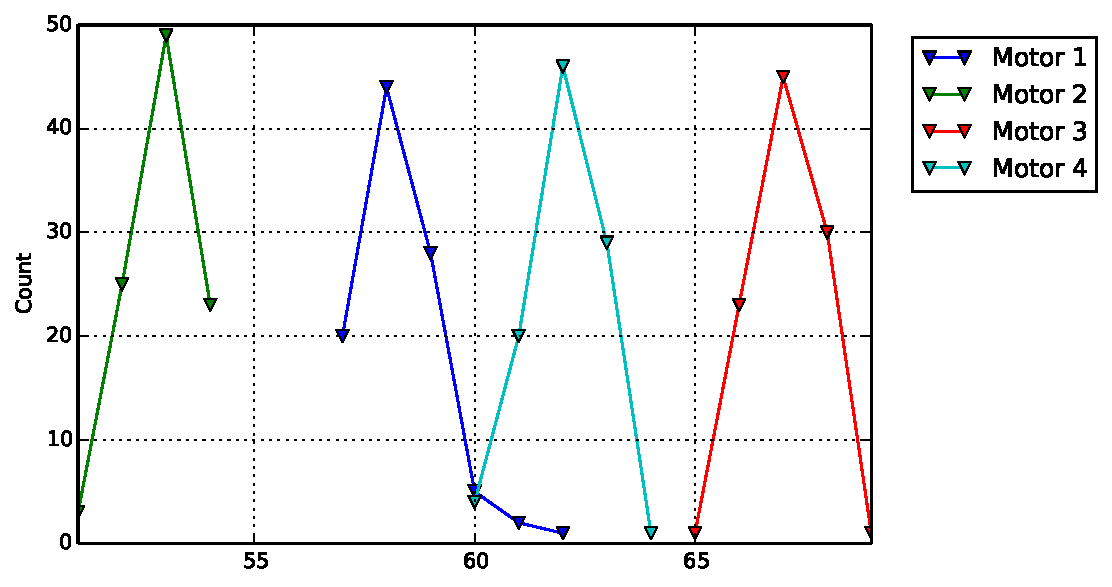
\includegraphics[scale=0.5]{graphics/test_graphs/Break_lineplot.pdf}
  \caption{Test data for motors, with the test \emph{Positive Brake Test}}
  \label{fig:cmp_all}
\end{figure}

\subsection{Test Conclusion}
Based on the data analysis of the test collected during the positive brake test, it can be concluded that \emph{motor 2} and \emph{4} are most suitable for usage in the system, as these two motors for fill the motor requirements and by such will fit into the system.

\section{Negative Brake Test}
This test examines the time each motor takes to brake, after it has been instructed to move a full rotation of 360\degree\ in a counter-clockwise direction. The result is given by the number degrees the motor has moved further than the instructed negative 360\degree . and will consider the consistency of each motor.

\subsection{Hypothesis} If a motor is set to move counter-clockwise 360\degree , the motor will move exactly -360 \degree .

\subsection{Test Procedure}
The test software is found in the file, \cfx{insert name of and ref to the test file, however this forces us to append the test source code as well!} As specified by the test structure, the test must be executed 100 times. This in implemented into the software, hence the program only needs to be executed once.
The software is designed to print the resulting degrees on  the \gls{nxt} screen, and the test conductor must therefore be ready to note down the results. To execute the test, the following list must be followed:
\begin{enumerate}
  \item Transfer the test software to the \gls{nxt} brick
  \item Fixate the test motor to a stable surface
  \item Connect test motor to the \gls{nxt} brick
  \item Check that the surface is stable and level
  \item Check that the motor is fixated
  \item Execute the test software once
  \item While program is running, note down the test results
\end{enumerate}

\subsection{Data analysis}\cfx{not reviewed}
As the expected resulted stated in the hypothesis is not meet, it is relevant to see if any of the uncertainties presented in \cref{sec:tech_uncertain}, could have affected the results for the test. Especial the uncertainties concerning \emph{Internal components} and \emph{Brake speed} is relevant, as these are central to this test situation. This is due to the fact that to measure the amount of degrees a motor have moved, the motor itself tells how many degrees it has moved. By such the test relies on that the internal motor components measurements are correct and if the internal components are incorrect this can affect the results of the test. Besides the internal components of the motor possible affect on the results, is a more direct uncertainty affecting the results, this uncertain is the braking speed of the motors. As the expected result of -360 degrees are not meet and all results for positive brake test presented in \cref{app:motor_test} are above expected result.

Based on the test data collected during the negative brake test, it is possible to draw certain conclusions. The data is presented in \cref{tbl:cmpl_negative_test_data} and \cref{fig:cmp_all_negative}, based on the data presented it is possible to determine that \emph{motor 4} is the best at braking and the most consistent motor and by such most suitable for usage in the system. Looking at the test data \emph{motor 1, 2} and \emph{3}, it is clear that \emph{motor 2} is the second best at braking and the second most consistent motor. Also \emph{Motor 1} is worst motor at braking, while \emph{motor 3} is better at braking it has a lower consistency.
\begin{figure}[ht]
  \centering
  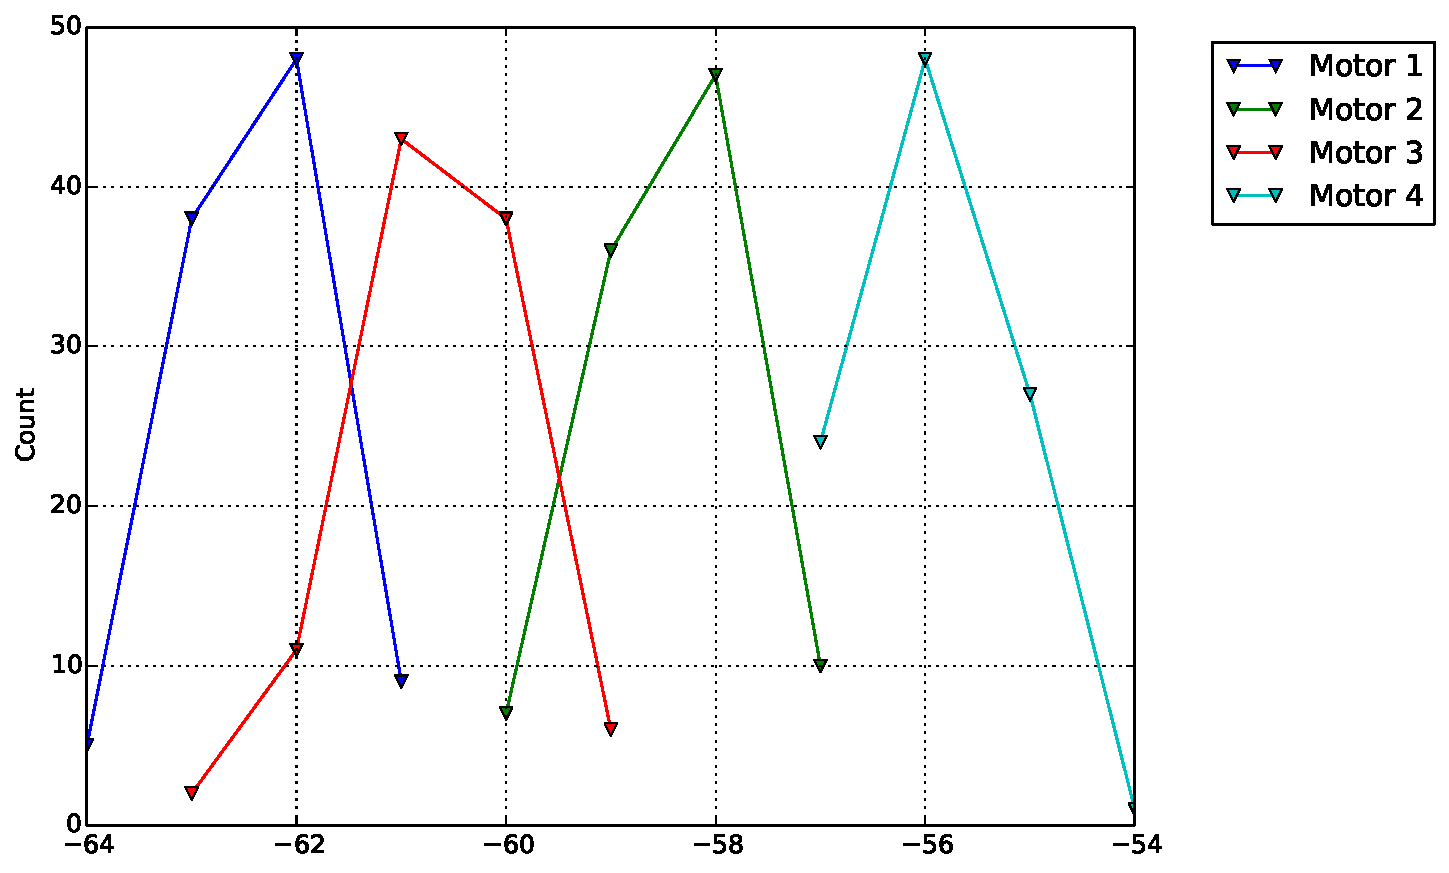
\includegraphics[scale=0.5]{graphics/test_graphs/Break_negative_lineplot.pdf}
  \caption{Test data for four motors, with the test \emph{Negative Brake Test}}
  \label{fig:cmp_all_negative}
\end{figure}

\subsection{Test Conclusion}
Based on the data analysis of the data collected during the negative brake test it can be concluded that \emph{motor 4} and \emph{motor 2} are most suitable for usage in the system, based on the stated motor requirements.

\section{Loaded Brake Test}
This test utilises the same test program \cfx{cref to the test program} as the \emph{Positive Brake Test}, which is again executed once, to run the total of 100 tests as specified to be required in the test structure. This test differs from the \emph{Positive Brake Test}, by having the motor connected to the rig used for the pointing device. Based on the \emph{Positive Brake Test}, the motors were not as precise as hypothesised. This test however is expected to have a more precise and less spread out result, as the load on the motor will help it break. The implementation of the rig also yields a result closer to practical use of the motor.

\subsection{Hypothesis} The motor will stay closer to the 360 degree mark and the spread out of the end results will be closer when it is attached to the rig, compared to the previous test in free space.

\subsection{Test Procedure}
The test software is found in the file, \cfx{insert name of and ref to the test file, however this forces us to append the test source code as well!} As specified by the test structure, the test must be executed 100 times. This in implemented into the software, hence the program only needs to be executed once.
The software is designed to print the resulting degrees on the \gls{nxt} screen, and the test conductor must therefore be ready to note down the results. To execute the test, the following list must be followed:
\begin{enumerate}
  \item Transfer the test software to the \gls{nxt} brick
  \item Attach the test motor to the rig
  \item Connect test motor to the \gls{nxt} brick
  \item Check that the surface and rig is stable and level
  \item Check that the motor is fixated
  \item Execute the test software once
  \item While program is running, note down the test results
\end{enumerate}

\subsection{Data analysis}\cfx{viewed}
The test is performed on motor 1 and when the data is compared to the other brake test in free space on the same motor, it can be seen that the degrees of which it overshoots the 360 mark is reduced by approximately 10\textdegree. The result matches the hypothesis as it predicted that very behaviour. The reason for this behaviour comes from the added stability from the rig and the higher friction between the gears. The other part of the hypothesis that mentions the reduced spread of end results is not true. In the same test where the number of degrees turned decreased, the spread of end results rose. The test in free space went from 417-422 degrees which covers a 6 degree width, whereas the weighted test went from 404-412 degrees which represents a width of 9.
%Se om det her også passer for de andre test resultater. Hvis spredningen bliver højere de andre steder også, så bliver jeg sur

\subsection{Test Conclusion}

